\documentclass{standalone}
\usepackage{tikz}
\usepackage{ctex,siunitx}
\setCJKmainfont{Noto Serif CJK SC}
\usepackage{tkz-euclide}
\usepackage{amsmath}
\usetikzlibrary{patterns, calc}
\usetikzlibrary {decorations.pathmorphing, decorations.pathreplacing, decorations.shapes,}
\begin{document}
\small
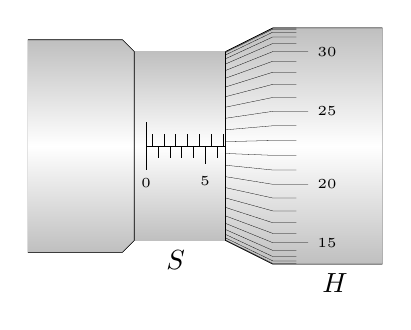
\begin{tikzpicture}[>=stealth,scale=1.5]
  \fill [top color=lightgray,bottom color=lightgray, middle color=white](-0.1,0.8)rectangle(0.7,-0.8);
  \draw[ultra thin](0,0)--++(0.7,0);
  \foreach \x in {0.1,0.2,0.3,0.4,0.6}
  {
    \draw[ultra thin](\x,0)--++(0,-0.1);
    \draw[ultra thin](\x+0.05,0)--++(0,0.1);
  }
  \draw[ultra thin](0.5,0)--++(0,-0.15)node[below=0.5mm]{\tiny 5};
  \draw[ultra thin](0,0.2)--++(0,-0.4)node[below]{\tiny 0};
  \draw[ultra thin](0.55,0)--++(0,0.1)(0.05,0)--++(0,0.1);
  \fill [top color=lightgray,bottom color=lightgray, middle color=white,draw,very thin](2,1)--(1.073,1)--++(-0.4,-0.2)--(0.673,-0.8)--++(0.4,-0.2)--(2,-1);
  \draw[very thin](0.673,-0.8)--(0.673,0.8);
  \fill [top color=lightgray,bottom color=lightgray, middle color=white,draw,very thin](-1,0.9)--(-0.2,0.9)--(-0.1,0.8)--(-0.1,-0.8)--(-0.2,-0.9)--(-1,-0.9);
  \node at (0.25,-0.8)[below]{$S$};
  \node at (1.6,-1)[below]{$H$};
  \foreach \x/\y in {-8/15,-3/20,2/25,7/30}
  {
    \draw[ultra thin](0.673,{0.8*sin(7.2*\x+2.7)})--(1.073,{sin(7.2*\x+2.7)})--++(0.3,0)node[right]{\tiny\y};
  }
  \foreach \x in {-12,-11,-10,-9,-7,-6,-5,-4,-2,-1,0,1,3,4,5,6,8,9,10,11,12}
  {
    \draw[ultra thin](0.673,{0.8*sin(7.2*\x+2.7)})--(1.073,{sin(7.2*\x+2.7)})--++(0.2,0);
  }
\end{tikzpicture}
\end{document}